\documentclass[conference]{IEEEtran}
\IEEEoverridecommandlockouts
\usepackage{cite}
\usepackage{graphicx}
\usepackage{booktabs}
\usepackage{array}
\usepackage{url}
\usepackage{amsmath}
\usepackage{multirow}
\raggedbottom
\hbadness=10000

\title{HERO-S: QPU-Aware Energy-Latency Orchestration for AIoT Intrusion Detection}

\author{\IEEEauthorblockN{Author Name(s) Omitted for Review}\IEEEauthorblockA{Institution Omitted for Review}}

\begin{document}
\maketitle

\begin{abstract}
AIoT intrusion-detection workflows increasingly span edge gateways, cloud AI accelerators, and optional remote quantum services. The practical systems question is whether each security task should remain at the edge, escalate to cloud inference, or enter a QPU-capable path under latency, queue-time, and energy constraints. This paper presents HERO-S, a QPU-aware edge-cloud orchestration framework for AIoT intrusion detection. HERO-S annotates tasks with alert severity, asset criticality, uncertainty, response deadline, backend queue time, route confidence, and energy estimates, then applies a constrained routing utility. We evaluate HERO-S on TON\_IoT, NSL-KDD, CICIDS2017, and IoT-23 over 30 seeds. The cloud model remains the upper-quality reference but violates a 2.5 ms/sample average gateway budget. Under that budget and 250 ms QPU queue time, HERO-S improves F1 over edge-only and over a closest classical uncertainty-cascade baseline on the three nontrivial datasets, maintains near-perfect edge performance on IoT-23, and reduces energy by 71.7--98.0\% relative to cloud-only routing. At 250 ms QPU queue time, HERO-S assigns all samples to edge/cloud routes, illustrating explicit queue-aware control of remote accelerator use.
\end{abstract}

\begin{IEEEkeywords}
AIoT security, intrusion detection, edge-cloud orchestration, QPU-aware scheduling, energy-aware routing.
\end{IEEEkeywords}

\section{Introduction}
AIoT security pipelines combine local telemetry collection, edge filtering, cloud-based machine learning, and specialized accelerators. Edge-computing and mobile-edge-computing studies motivate splitting latency-sensitive computation across devices, gateways, and cloud resources \cite{shi2016edge,mach2017mec}. Near-term QPUs add a possible remote route for quantum kernels and variational methods \cite{preskill2018nisq,havlicek2019supervised,schuld2019qml,cerezo2021vqa}. This creates a route-selection problem: the defender must decide when a remote quantum-capable path is worth its added delay and energy.

HERO-S addresses this route-selection layer. Current QPU-compatible classifiers are evaluated as candidate routes, and every route is scored by expected quality, deadline, backend queue time, confidence, and energy. This framing separates the upper-quality cloud IDS reference from the feasible policies that must satisfy a gateway latency budget.

The contributions are: (1) an AIoT edge-cloud-QPU intrusion-detection formulation; (2) HERO-Scheduler, a security-aware route-selection policy using severity, asset criticality, uncertainty, confidence gates, deadlines, queue time, and energy estimates; (3) a 30-seed evaluation on four real IDS datasets; (4) quantitative comparison with a closest classical uncertainty-cascade baseline, including route-call rates, SLA violations, energy, and energy-delay product (EDP); and (5) a transparent QPU-proxy methodology that separates scheduler-scale proxy results from small Qiskit quantum-kernel feasibility runs.

\section{Threat and Workload Model}
\subsection{Deployment Model}
HERO-S assumes an AIoT edge-cloud continuum. IoT devices produce packet or flow telemetry, edge gateways perform normalization and low-cost filtering, cloud CPU/GPU resources run stronger IDS models, and a remote QPU service is available as an optional path. The QPU is not placed on the IoT device; it is a scarce remote service with queue time, shot budget, execution latency, and modeled infrastructure energy.

The deployment is compatible with common AIoT data planes. Sensors and gateways may export flow summaries through MQTT, CoAP, HTTP, or a site-local message broker. The orchestrator consumes normalized flow records and backend state, not raw packet payloads. Edge devices therefore remain lightweight while cloud and QPU-capable routes are used only when their expected security utility justifies additional delay and energy.

\subsection{Attacker, Defender, and Metadata}
The defender observes flow telemetry from AIoT devices and gateways. The attacker may generate denial-of-service, scanning, brute-force, botnet, backdoor, infiltration, or web-attack traffic. Each task node records model and security metadata used by the scheduler: severity raises priority for likely attacks, asset criticality distinguishes controllers from low-risk devices, uncertainty triggers escalation when edge inference is ambiguous, confidence checks whether the target route is reliable enough, deadlines penalize slow routes, queue time captures remote-backend delay, and energy prevents expensive routes without expected utility gain. In the experiments, severity is derived from the edge attack probability, uncertainty is one minus edge confidence, asset criticality is assigned on a 1--5 scale to represent heterogeneous devices, and deadlines are sampled from representative edge-response classes.

\section{HERO-S Architecture and Scheduler}
Fig.~\ref{fig:arch} shows the system architecture. HERO-S has an ingestion layer, an edge preprocessing and lightweight IDS layer, a cloud AI layer, a QPU-capable analysis path, and a telemetry/scheduler control plane.

\begin{figure*}[t]
\centering
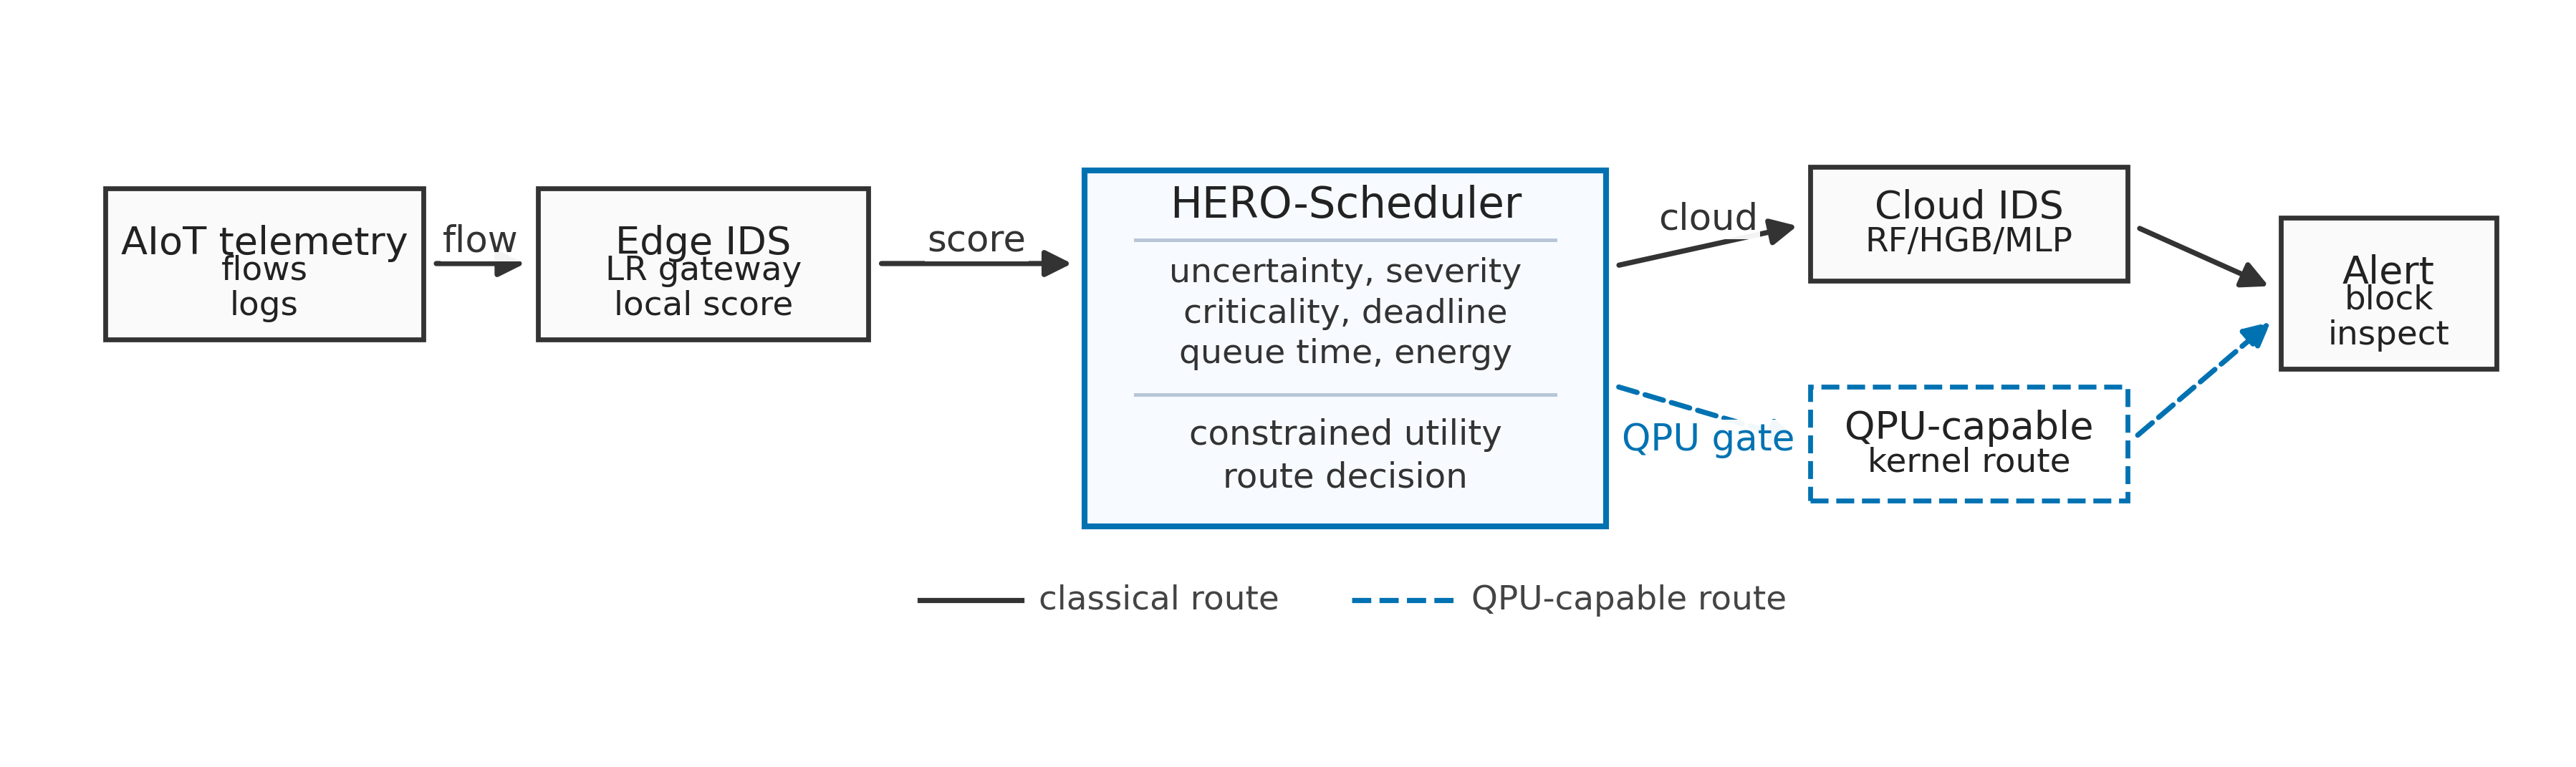
\includegraphics[width=0.92\textwidth]{figures/hero_s_architecture.png}
\caption{HERO-S edge-cloud-QPU architecture. Flow telemetry is first handled by the edge; uncertain or high-risk cases may be escalated to cloud inference or a QPU-capable route depending on deadline, confidence, queue time, and energy.}
\label{fig:arch}
\end{figure*}

\subsection{Utility Function}
For each ready task $v$, HERO-Scheduler evaluates candidate route $r$ by
\begin{equation}
\begin{split}
score(r,v) &= \alpha Q(v,r) + \beta R(v) - \gamma E(v,r) \\
&\quad - \delta L(v,r) - \eta W(r) - \zeta S(v,r),
\end{split}
\end{equation}
where $Q$ is expected quality gain, $R$ is security risk, $E$ is energy, $L$ is latency, $W$ is queue time, and $S$ is predicted SLA violation. Security risk is severity times asset criticality and false-negative cost. Unless otherwise stated, HERO-S uses $\alpha=2.0$, $\beta=1.5$, $\gamma=0.001$, $\delta=0.015$, $\eta=0.01$, and $\zeta=1.0$. These values are fixed across datasets and set quality and security risk as dominant terms, while energy, latency, queue time, and SLA violations act as penalties. The scheduler uses edge routes for high-confidence or budget-tight samples, cloud routes for stronger classical inference when confidence and latency permit, and QPU-capable routes only when uncertainty, risk, queue time, and confidence justify the additional cost.

HERO-S also applies two safety gates. First, cloud escalation requires edge uncertainty at least 0.08 and cloud-route confidence at least 0.70, followed by an average 2.5 ms/sample latency-budget check. Second, a QPU-capable route must win the utility score and must have a confidence margin over the edge/cloud alternatives; otherwise the task falls back to the best feasible classical route. These gates make fallback behavior an explicit part of the algorithm.

\subsection{Baselines and Complexity}
We compare HERO-S with four routing policies. Edge-only performs minimum-energy gateway inference with no escalation. Cloud-only is the upper-quality classical reference but violates the average budget. Static QPU is a stress-test baseline that always takes the QPU-capable route. The closest classical baseline is an uncertainty cascade: it first runs the edge model and escalates to cloud when edge uncertainty is at least 0.25; it has no security metadata, QPU awareness, queue term, or energy term.

HERO-Scheduler processes ready tasks in dependency order, filters infeasible routes, estimates each route's quality gain and cost from the telemetry state, scores all feasible routes, dispatches the task, and updates backend state. The scheduling pass costs $O(|V||R|)$ time and $O(|R|)$ per-task memory for $|V|$ tasks and $|R|$ routes. In the evaluated system $|R|=3$ (edge, cloud, QPU-capable), so the scheduler is lightweight relative to IDS inference and remote backend delay.


\section{Experimental Methodology}
\subsection{Datasets and Sampling}
Table~\ref{tab:datasets} summarizes the datasets. TON\_IoT and IoT-23 provide IoT/IIoT traffic \cite{alsaedi2020toniot,garcia2020iot23}; CICIDS2017 provides a modern IDS benchmark \cite{sharafaldin2018toward,sharafaldin2018detailed}; NSL-KDD is retained as a reproducible legacy baseline \cite{tavallaee2009kdd}. TON\_IoT is stratified-sampled to 20,000 rows. CICIDS2017 is sampled from all eight daily parquet files with up to 5,000 rows per file, preserving coverage across benign, DDoS, port scan, infiltration, web attack, botnet, and brute-force traffic. NSL-KDD uses the standard train/test files with stratified caps. IoT-23 drops IP, UID, detailed label, and scenario fields to reduce leakage; because the selected subset is easy, it is treated as venue-alignment validation rather than the hardest benchmark.

\begin{table}[t]
\caption{Datasets used in the 30-seed evaluation.}
\label{tab:datasets}
\centering
\scriptsize
\begin{tabular}{lrrrrr}
\toprule
Dataset & Samples & Feat. & Normal & Attack & Ratio \\
\midrule
TON\_IoT & 20,000 & 40 & 10,000 & 10,000 & 0.500 \\
NSL-KDD & 7,000 & 41 & 3,500 & 3,500 & 0.500 \\
CICIDS2017 & 40,000 & 78 & 25,818 & 14,182 & 0.355 \\
IoT-23 & 10,035 & 15 & 7,200 & 2,835 & 0.283 \\
\bottomrule
\end{tabular}
\end{table}

\subsection{IDS Models and QPU-Compatible Route}
Classical IDS baselines are Logistic Regression, RBF-SVM, Random Forest, Histogram Gradient Boosting, and MLP. The edge route uses Logistic Regression because it has a compact linear decision rule and small memory footprint suitable for gateway inference, while the cloud route uses Random Forest as a stronger ensemble reference with larger model state; Table~\ref{tab:ids} reports the full comparison. Scheduler-scale QPU behavior is represented by a four-feature reduced-kernel proxy. The proxy represents the feature-reduced interface that a QPU-compatible kernel path would occupy in the routing graph. We also run small Qiskit quantum-kernel subsets on TON\_IoT and NSL-KDD using 16 training samples, 8 test samples, 256 shots, and 3 seeds \cite{qiskit,aer}.

The proxy exercises the route that a future QPU kernel implementation would occupy in the orchestration graph. When its expected utility is below classical inference, HERO-S falls back to edge or cloud execution and preserves scarce backend capacity.

\subsection{Metrics, Energy, and Statistical Tests}
Metrics include accuracy, precision, recall, F1, ROC-AUC, PR-AUC, FPR, FNR, latency/sample, energy/sample, EDP, route-call rates, sampled-deadline violation rate, and average-budget violation. We report mean and standard deviation over 30 seeds and use paired Wilcoxon signed-rank tests for HERO-S versus edge-only and versus the uncertainty cascade. The 2.5 ms/sample constraint is a representative average gateway compute budget used to stress-test latency-sensitive edge operation. Edge-computing and MEC surveys motivate pushing latency-sensitive services toward nearby resources for highly responsive operation \cite{satyanarayanan2017edge,mao2017mec}; we also report sampled-deadline violation rates with per-flow deadlines drawn from 5--100 ms response classes.

CPU/GPU energy uses RAPL/NVML counters when available and otherwise a labeled fallback model. QPU infrastructure energy is modeled for scheduling sensitivity because direct facility telemetry is outside the current artifact. Static QPU routing is therefore reported as a stress-test baseline. The modeled route costs are 1.2 ms and 0.0227 J for edge CPU, 6.0 ms and 1.296 J for cloud CPU/GPU, and 75--325 ms plus 1800 J for the QPU-capable path depending on queue time.

\begin{table}[t]
\caption{Route-cost and telemetry assumptions.}
\label{tab:energy_source}
\centering
\scriptsize
\resizebox{\columnwidth}{!}{%
\begin{tabular}{@{}p{0.22\columnwidth}p{0.18\columnwidth}p{0.18\columnwidth}p{0.32\columnwidth}@{}}
\toprule
Route & Lat. & Energy & Source \\
\midrule
Edge CPU & 1.2 ms & 0.0227 J & RAPL if available; fallback model otherwise. \\
Cloud CPU/GPU & 6.0 ms & 1.296 J & NVML/RAPL if available; fallback model otherwise. \\
QPU-capable & 75--325 ms & 1800 J & Modeled infrastructure sensitivity only. \\
\bottomrule
\end{tabular}}
\end{table}

\section{Results}
\subsection{IDS Quality and Proxy Limits}
Table~\ref{tab:ids} gives the complete classical baseline comparison over 30 seeds. Strong classical models, especially RF and HGB, are the best quality references on the evaluated datasets. These results motivate QPU-aware route admission: QPU-capable execution is selected only when its expected utility exceeds the edge and cloud alternatives.

\begin{table*}[t]
\caption{IDS baseline comparison over 30 seeds. Values are means; Proxy F1 also reports standard deviation because the reduced-kernel route is used in the scheduler-scale audit.}
\label{tab:ids}
\centering
\begingroup
\tiny
\setlength{\tabcolsep}{3.0pt}
\renewcommand{\arraystretch}{0.84}
\begin{tabular}{@{}llccccccc@{}}
\toprule
Dataset & Model & Acc. & F1 & Recall & FPR & FNR & ROC-AUC & PR-AUC \\
\midrule
TON\_IoT & LR & 0.944 & 0.945 & 0.966 & 0.079 & 0.034 & 0.991 & 0.991 \\
 & RBF-SVM & 0.973 & 0.973 & 0.968 & 0.022 & 0.032 & 0.982 & 0.986 \\
 & RF & 0.994 & 0.994 & 0.996 & 0.007 & 0.004 & 1.000 & 1.000 \\
 & HGB & 0.995 & 0.995 & 0.995 & 0.006 & 0.005 & 1.000 & 1.000 \\
 & MLP & 0.978 & 0.978 & 0.968 & 0.012 & 0.032 & 0.994 & 0.994 \\
 & Proxy & 0.889 & 0.891$\pm$0.030 & 0.906 & 0.128 & 0.094 & 0.916 & 0.899 \\
\midrule
NSL-KDD & LR & 0.772 & 0.732 & 0.620 & 0.076 & 0.380 & 0.858 & 0.876 \\
 & RBF-SVM & 0.789 & 0.747 & 0.622 & 0.044 & 0.378 & 0.893 & 0.908 \\
 & RF & 0.801 & 0.760 & 0.630 & 0.027 & 0.370 & 0.961 & 0.956 \\
 & HGB & 0.809 & 0.772 & 0.646 & 0.027 & 0.354 & 0.952 & 0.946 \\
 & MLP & 0.789 & 0.755 & 0.652 & 0.075 & 0.348 & 0.873 & 0.889 \\
 & Proxy & 0.763 & 0.712$\pm$0.013 & 0.586 & 0.061 & 0.414 & 0.829 & 0.874 \\
\midrule
CICIDS2017 & LR & 0.888 & 0.892 & 0.929 & 0.153 & 0.071 & 0.944 & 0.934 \\
 & RBF-SVM & 0.906 & 0.911 & 0.956 & 0.143 & 0.044 & 0.960 & 0.944 \\
 & RF & 0.991 & 0.991 & 0.990 & 0.009 & 0.010 & 0.999 & 0.998 \\
 & HGB & 0.995 & 0.995 & 0.996 & 0.005 & 0.004 & 0.999 & 0.999 \\
 & MLP & 0.952 & 0.953 & 0.973 & 0.068 & 0.027 & 0.989 & 0.987 \\
 & Proxy & 0.744 & 0.679$\pm$0.108 & 0.567 & 0.078 & 0.433 & 0.804 & 0.840 \\
\midrule
IoT-23 & LR & 0.999 & 0.999 & 0.999 & 0.001 & 0.001 & 1.000 & 0.999 \\
 & RBF-SVM & 1.000 & 0.999 & 0.999 & 0.000 & 0.001 & 1.000 & 1.000 \\
 & RF & 1.000 & 1.000 & 0.999 & 0.000 & 0.001 & 1.000 & 1.000 \\
 & HGB & 1.000 & 1.000 & 0.999 & 0.000 & 0.001 & 1.000 & 1.000 \\
 & MLP & 0.999 & 0.999 & 0.998 & 0.000 & 0.002 & 0.999 & 0.999 \\
 & Proxy & 0.997 & 0.997$\pm$0.001 & 0.994 & 0.000 & 0.006 & 1.000 & 1.000 \\
\bottomrule
\end{tabular}
\endgroup
\end{table*}


\begin{figure}[t]
\centering
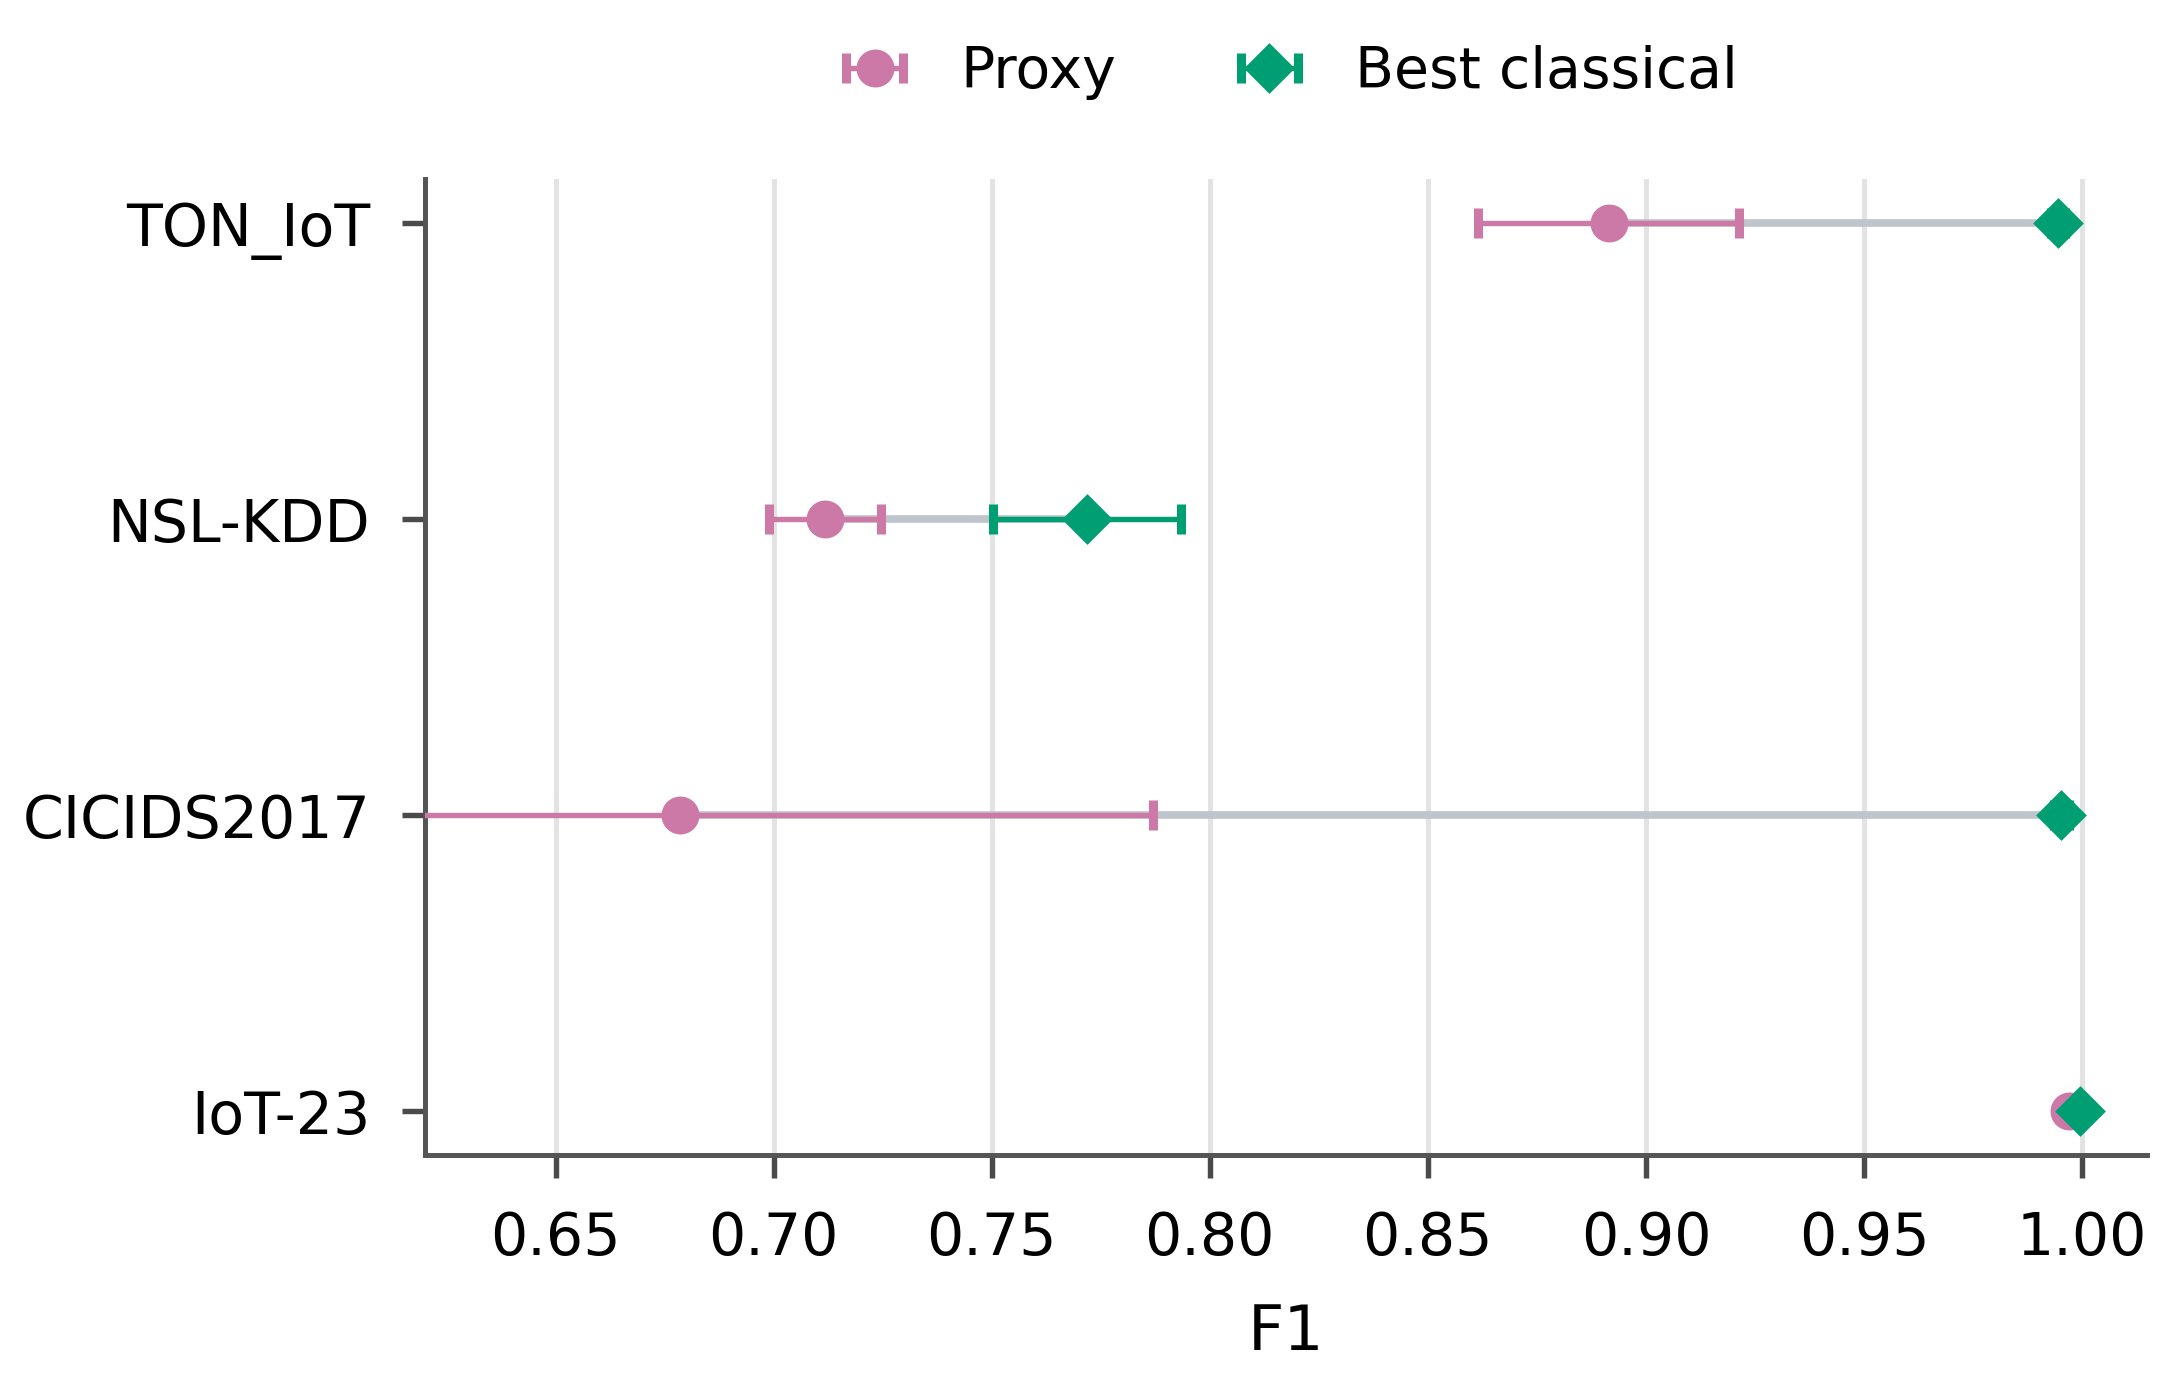
\includegraphics[width=\columnwidth]{figures/all_datasets_ids_f1.png}
\caption{F1 scores for the best classical IDS model and the reduced-kernel proxy.}
\label{fig:ids}
\end{figure}

The reduced-kernel proxy is weakest and least stable on CICIDS2017 (F1 $0.679\pm0.108$), whereas IoT-23 is nearly saturated. This instability motivates confidence-gated QPU-capable routing. HERO-S therefore uses the proxy route for selected uncertain/high-risk cases at low queue time and falls back to classical routes when confidence, queue, or latency conditions are unfavorable.

\subsection{Closest-Baseline Scheduler Comparison}
Table~\ref{tab:scheduler} addresses the main orchestration question under deadline and queue constraints. Under an unconstrained setting, cloud-only routing gives the strongest F1 on TON\_IoT, NSL-KDD, and CICIDS2017. Under a 2.5 ms/sample average gateway budget, however, cloud-only routing at 6.0 ms/sample is infeasible. At 250 ms QPU queue time, HERO-S satisfies the average budget, avoids QPU calls, improves F1 over both edge-only and the uncertainty cascade on the three nontrivial datasets, and achieves only marginal additional F1 on the near-saturated IoT-23 setting.

\begin{table*}[t]
\caption{Deadline-constrained scheduler comparison at 250 ms QPU queue time. F1 values are 30-seed means; HERO-S F1 also reports standard deviation. Cloud-only is an upper-quality reference but violates the 2.5 ms/sample average budget.}
\label{tab:scheduler}
\centering
\scriptsize
\resizebox{\textwidth}{!}{%
\begin{tabular}{lcccccccccc}
\toprule
Dataset & Edge F1 & Cascade F1 & HERO-S F1 & Cloud F1 & HERO lat. & HERO energy & EDP & Edge/Cloud/QPU & Deadl. viol. & $p$ vs Cascade \\
\midrule
TON\_IoT & 0.945 & 0.979 & 0.990$\pm$0.003 & 0.994 & 1.878 ms & 0.203 J & 0.383 & 0.859/0.141/0.000 & 0.021 & $1.86\times10^{-9}$ \\
NSL-KDD & 0.732 & 0.727 & 0.747$\pm$0.014 & 0.760 & 1.541 ms & 0.113 J & 0.175 & 0.929/0.071/0.000 & 0.011 & $3.54\times10^{-8}$ \\
CICIDS2017 & 0.892 & 0.937 & 0.946$\pm$0.005 & 0.991 & 2.498 ms & 0.367 J & 0.917 & 0.730/0.270/0.000 & 0.040 & $4.66\times10^{-8}$ \\
IoT-23 & 0.999 & 0.999 & 1.000$\pm$0.001 & 1.000 & 1.211 ms & 0.0256 J & 0.031 & 0.998/0.002/0.000 & 0.00045 & $1.60\times10^{-2}$ \\
\bottomrule
\end{tabular}}
\end{table*}

\begin{figure}[t]
\centering
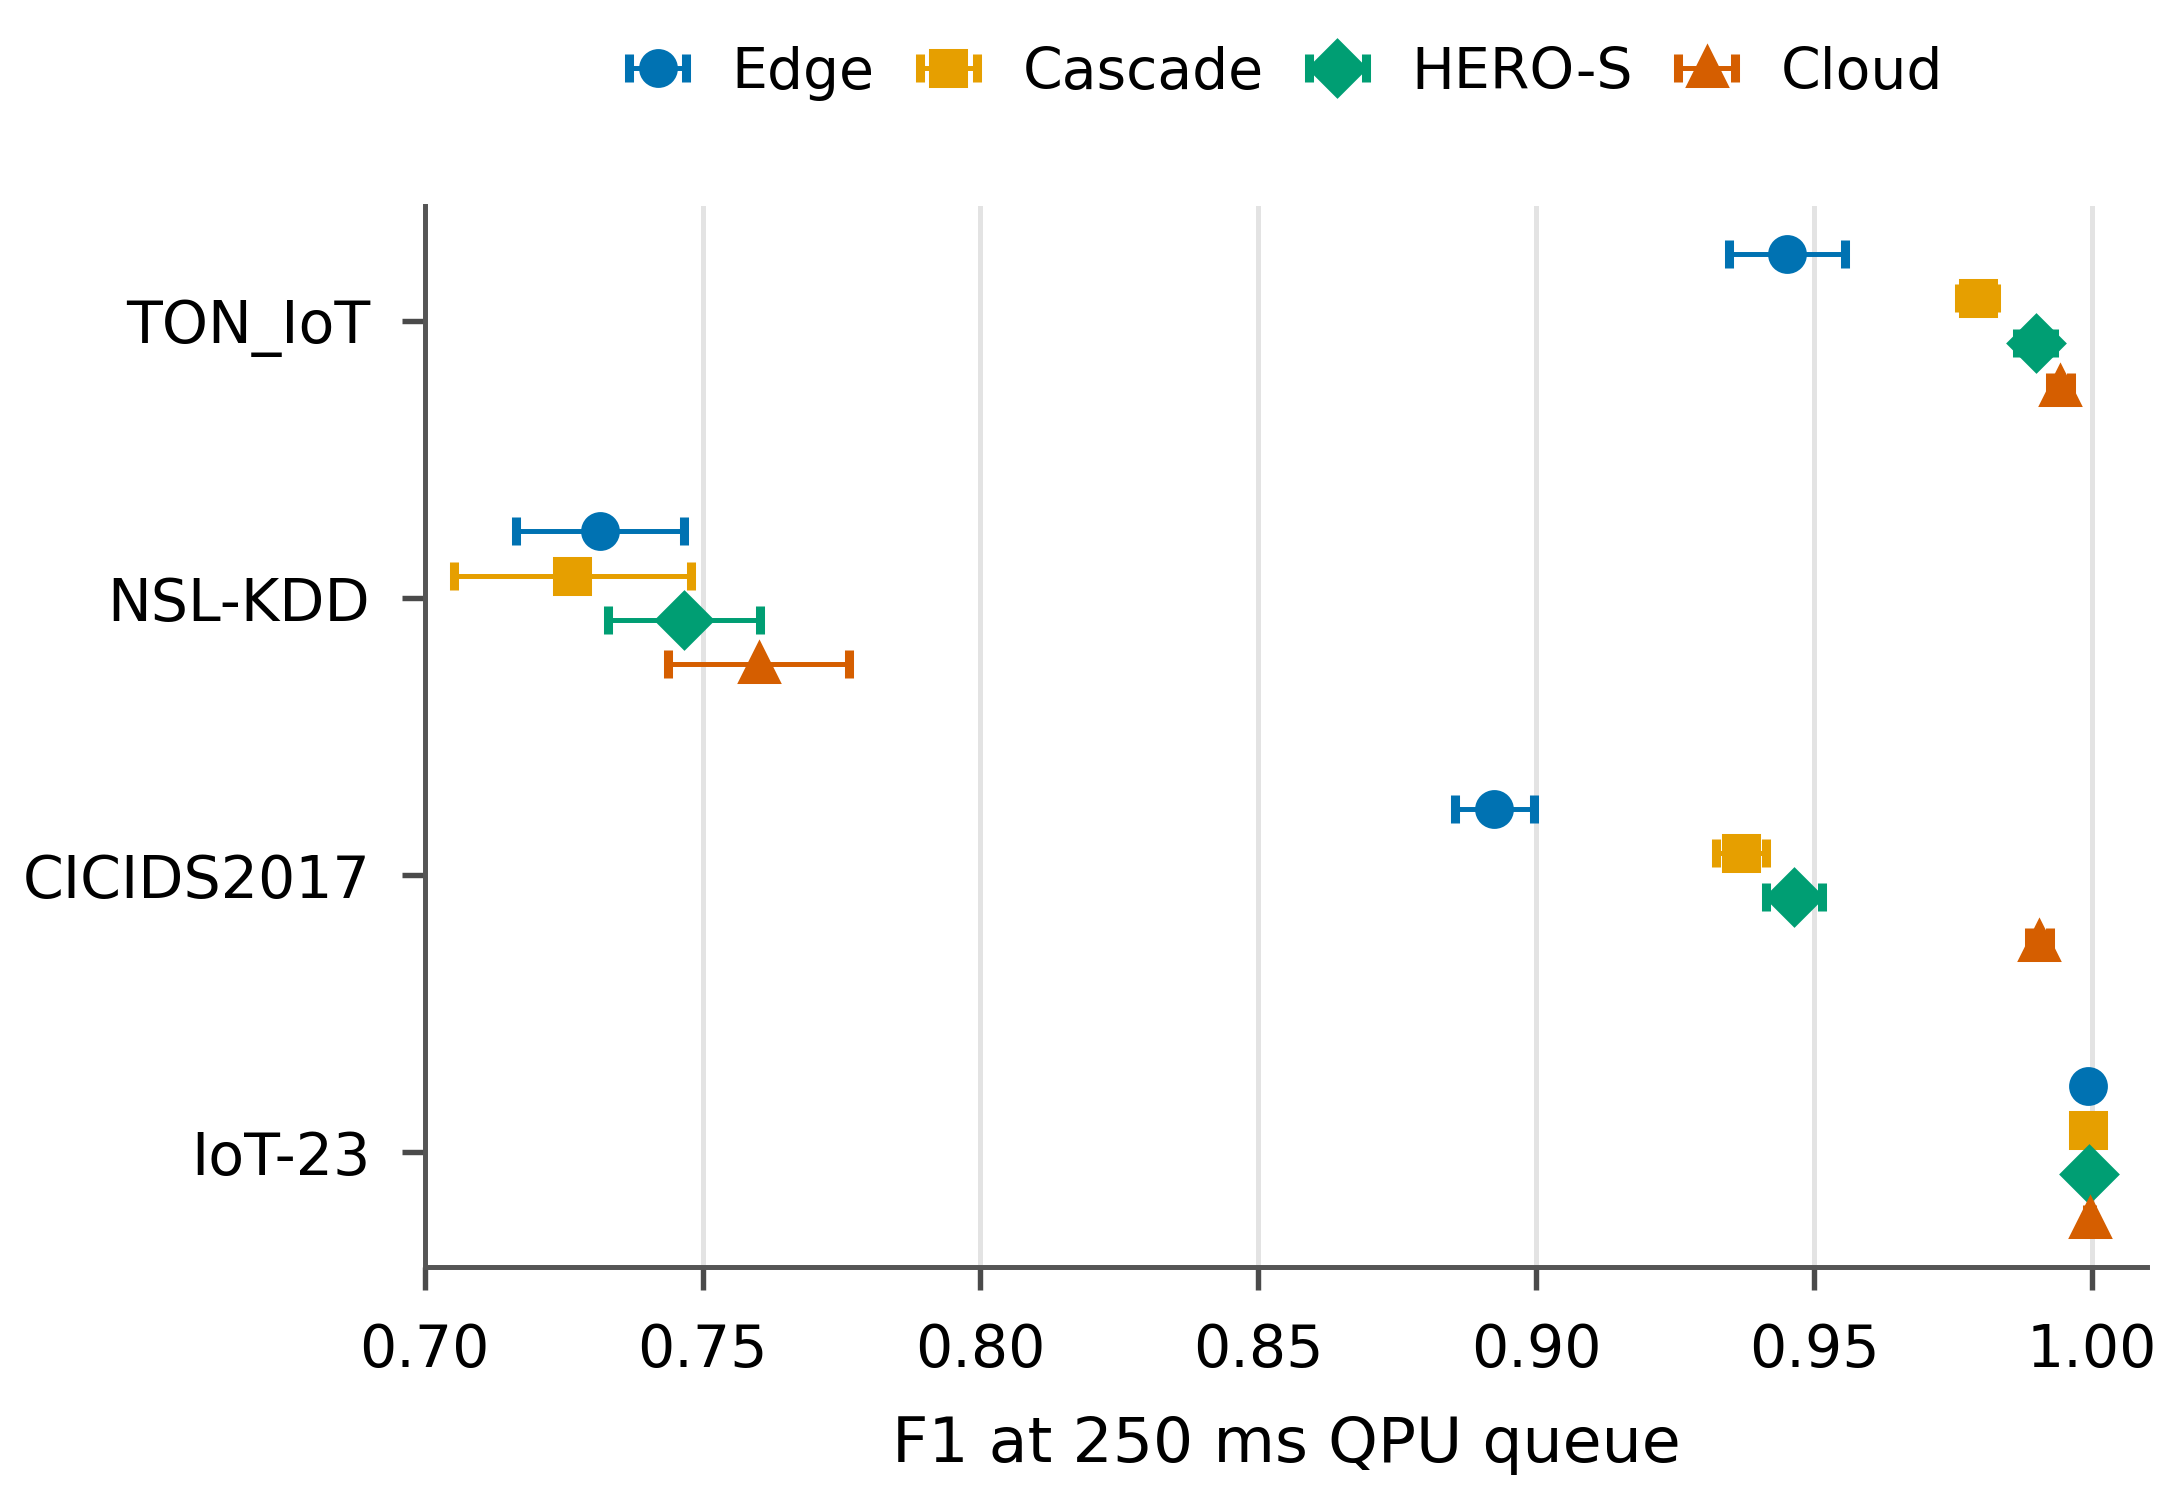
\includegraphics[width=\columnwidth]{figures/scheduler_baseline_comparison.png}
\caption{Closest-baseline comparison at 250 ms QPU queue time. HERO-S improves over edge-only and the uncertainty cascade while remaining below the average latency budget.}
\label{fig:baseline}
\end{figure}

\begin{figure}[t]
\centering
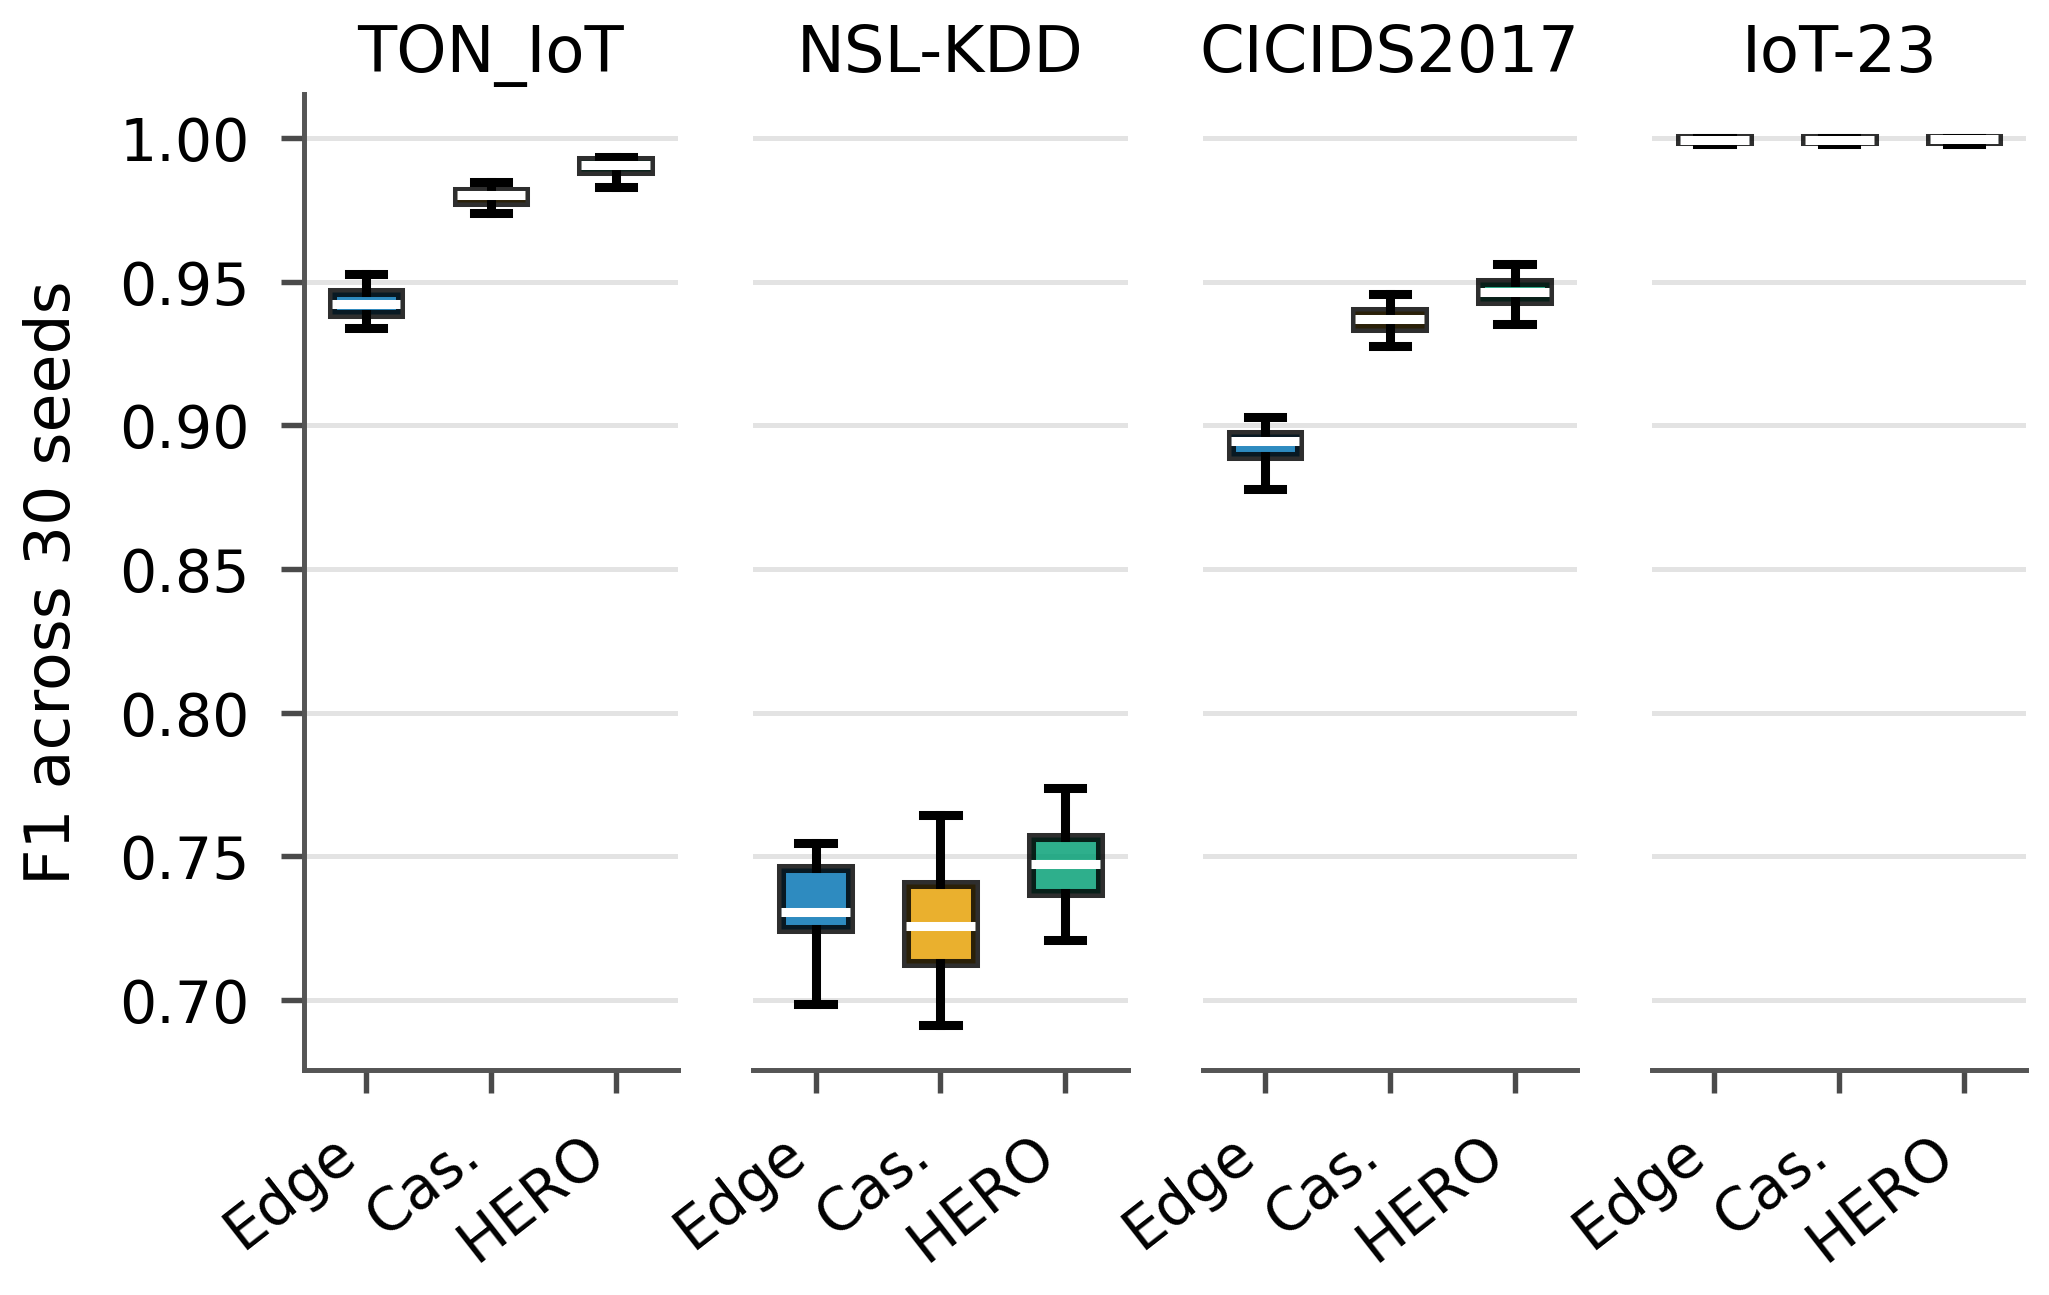
\includegraphics[width=\columnwidth]{figures/hero_s_f1_boxplot.png}
\caption{Thirty-seed F1 distributions for edge-only, uncertainty cascade, and HERO-S at 250 ms QPU queue time.}
\label{fig:boxplot}
\end{figure}

NSL-KDD illustrates a limitation of fixed uncertainty cascades: the 0.25 rule escalates a small subset whose cloud predictions do not consistently improve the edge decision, so cascade F1 can fall below edge-only even though the cloud model is stronger on average. The cascade threshold is a reasonable classical design choice, but it does not consider cloud confidence, security risk, or backend state. HERO-S uses a lower uncertainty trigger (0.08) only together with a cloud-confidence gate ($\geq$0.70), security-risk weighting, and an average-budget check, so lower uncertainty alone does not guarantee cloud escalation. Route-call rates in Table~\ref{tab:scheduler} also identify where the gains originate. At 250 ms queue time, QPU call rate is zero on all datasets because the proxy has lower expected utility than the classical alternatives under the queue and latency budget. The quality gains come from selective edge-cloud routing: HERO-S sends 14.1\% of TON\_IoT samples, 7.1\% of NSL-KDD samples, 27.0\% of CICIDS2017 samples, and 0.2\% of IoT-23 samples to cloud inference. Fig.~\ref{fig:boxplot} shows that the 30-seed distributions follow the same pattern. On IoT-23, all policies are already near perfect; the numerical F1 difference is operationally negligible, and HERO-S keeps the route mix almost entirely at the edge.

\subsection{Energy-Latency Tradeoff}
Edge-only remains the lowest-energy baseline. HERO-S trades additional joules for recovered detection quality while satisfying the average latency budget. Compared with cloud-only routing, HERO-S reduces energy by 84.4\% on TON\_IoT, 91.3\% on NSL-KDD, 71.7\% on CICIDS2017, and 98.0\% on IoT-23. Its EDP remains far below cloud-only: 0.383, 0.175, 0.917, and 0.031 versus 7.776 for cloud-only. Static QPU routing has EDP $5.85\times10^5$ at 250 ms queue time and serves as the stress-test baseline.

\begin{figure}[t]
\centering
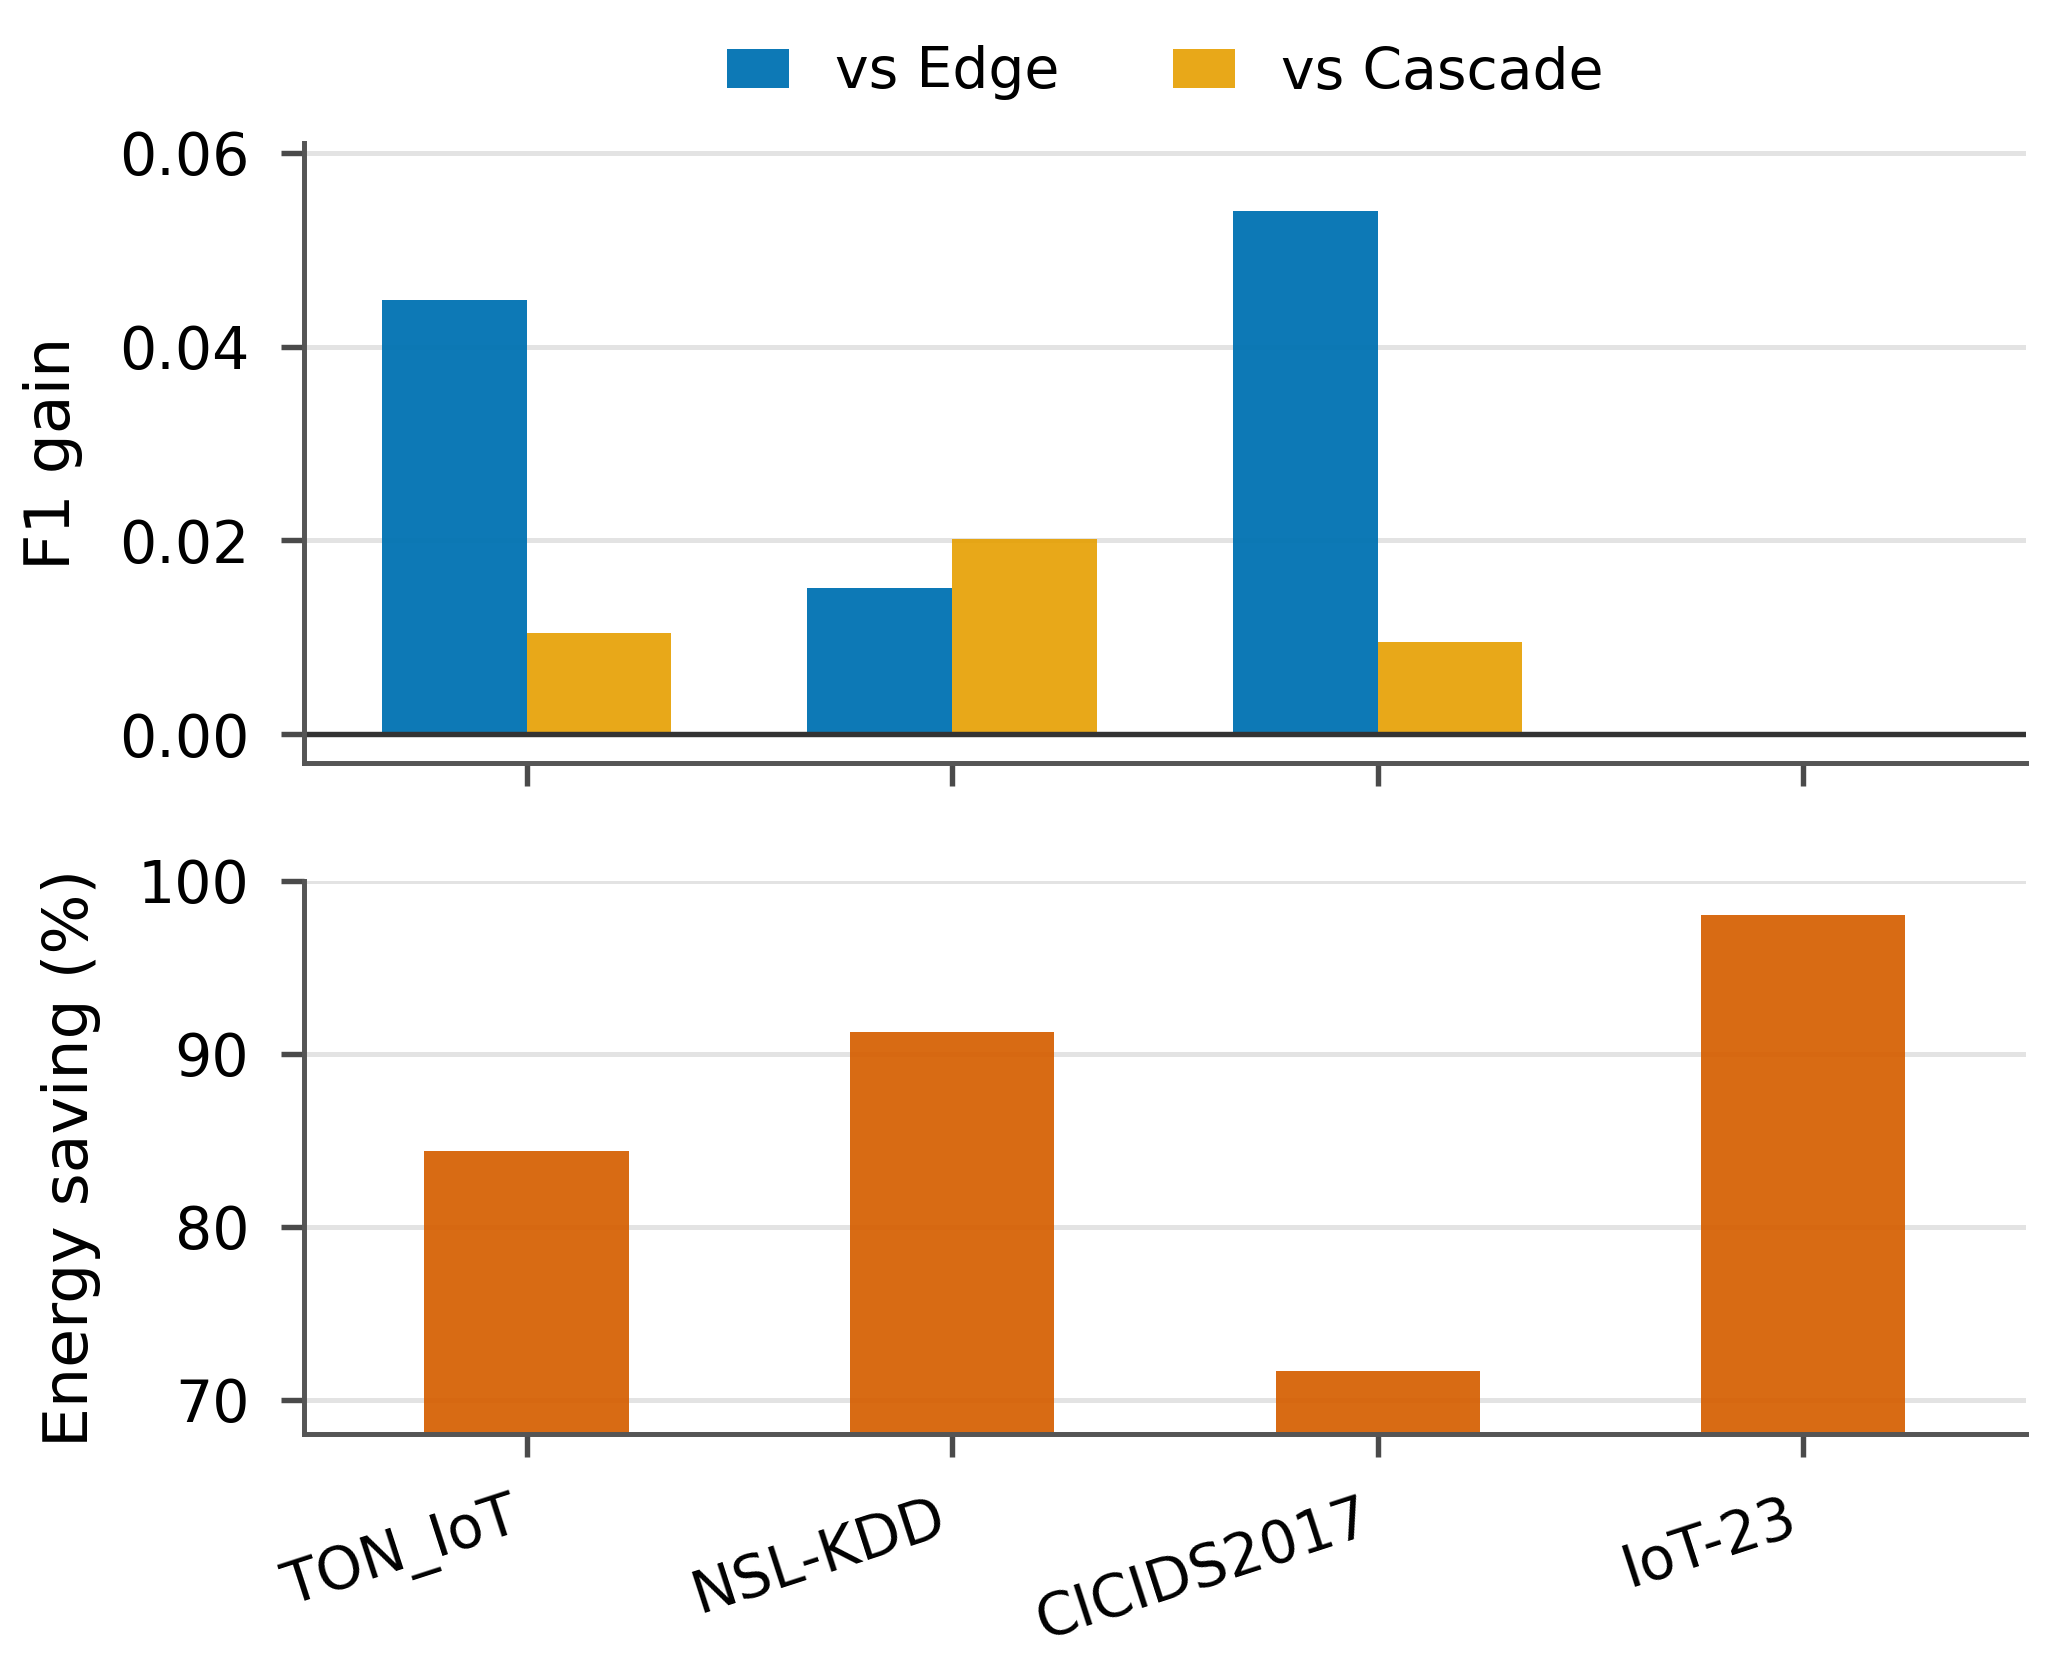
\includegraphics[width=\columnwidth]{figures/deadline_constrained_tradeoff.png}
\caption{F1 gain and energy savings under the deadline-constrained setting. HERO-S pays more energy than edge-only but remains far below cloud-only energy.}
\label{fig:deadline}
\end{figure}

\begin{figure}[t]
\centering
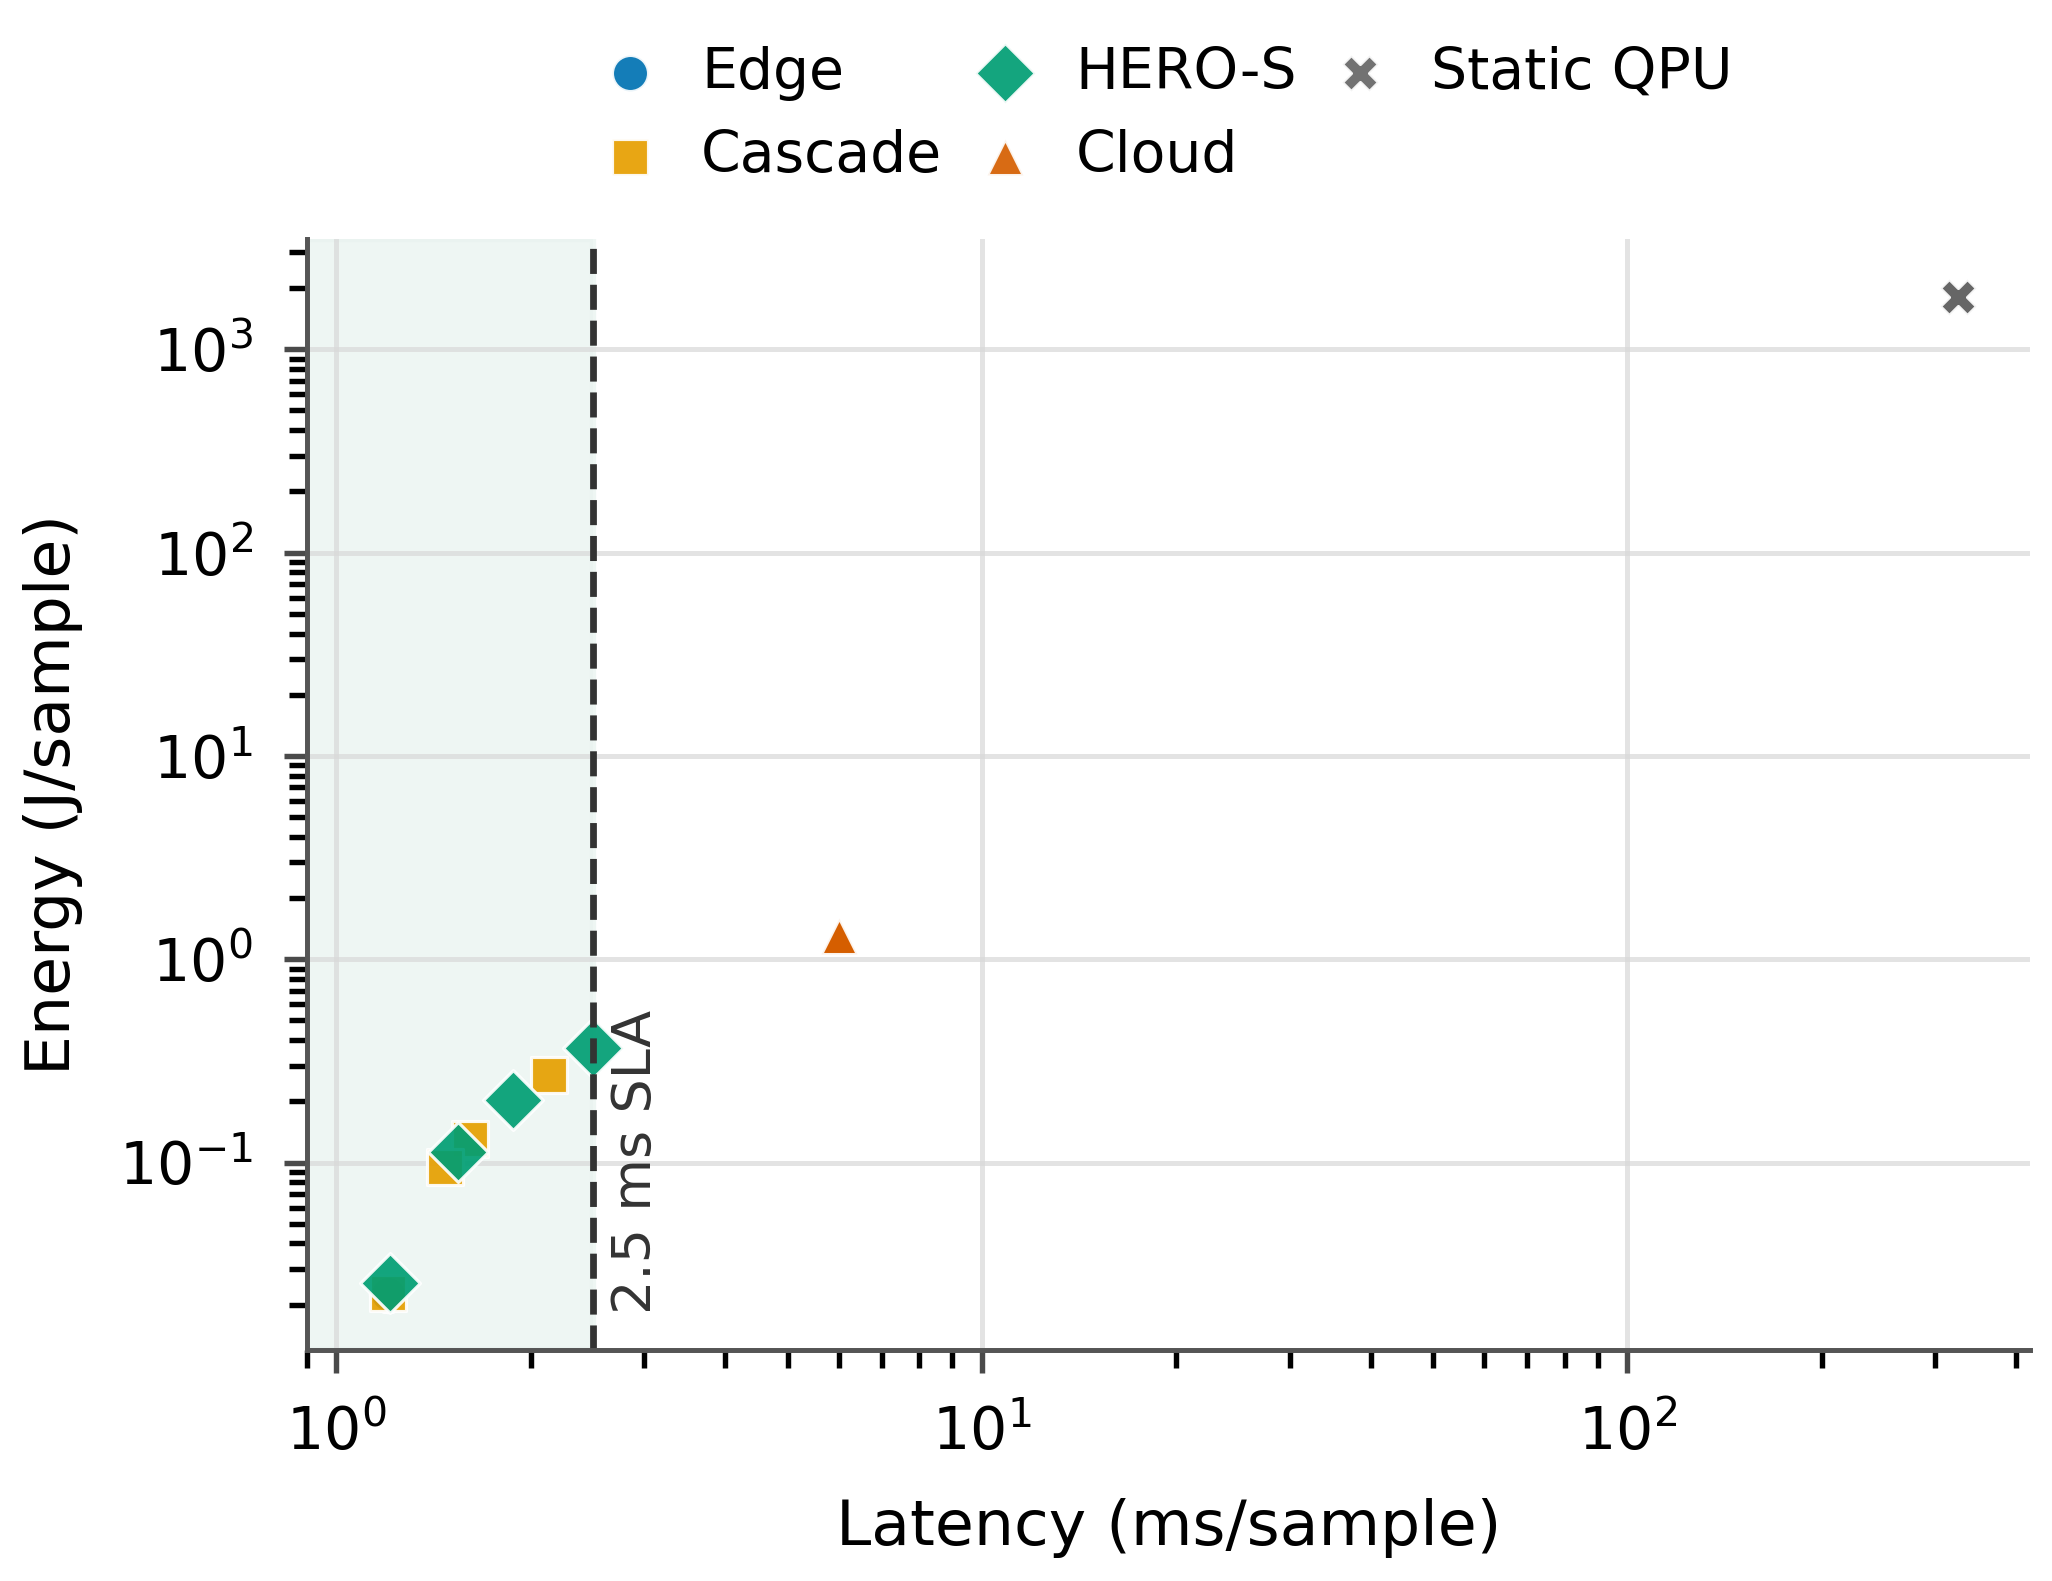
\includegraphics[width=\columnwidth]{figures/scheduler_energy_latency_tradeoff.png}
\caption{Energy-latency policy tradeoff. The dashed line marks the 2.5 ms/sample average budget.}
\label{fig:energy}
\end{figure}

\subsection{QPU Queue Sensitivity}
Fig.~\ref{fig:queue} shows that QPU use changes with backend queue time. At zero queue, HERO-S invokes the QPU-capable path for 0.001 of TON\_IoT samples, 0.010 of NSL-KDD samples, 0.000 of CICIDS2017 samples, and almost none on IoT-23. At an intermediate 50 ms queue, these rates drop to 0.0005 on TON\_IoT, 0.0037 on NSL-KDD, and zero or nearly zero on the other datasets. At 250 ms, QPU calls drop to zero on all datasets. This monotonic response follows directly from the queue term: when the proxy route lacks sufficient confidence or queue conditions are poor, HERO-S selects the edge or cloud route.

\begin{figure}[t]
\centering
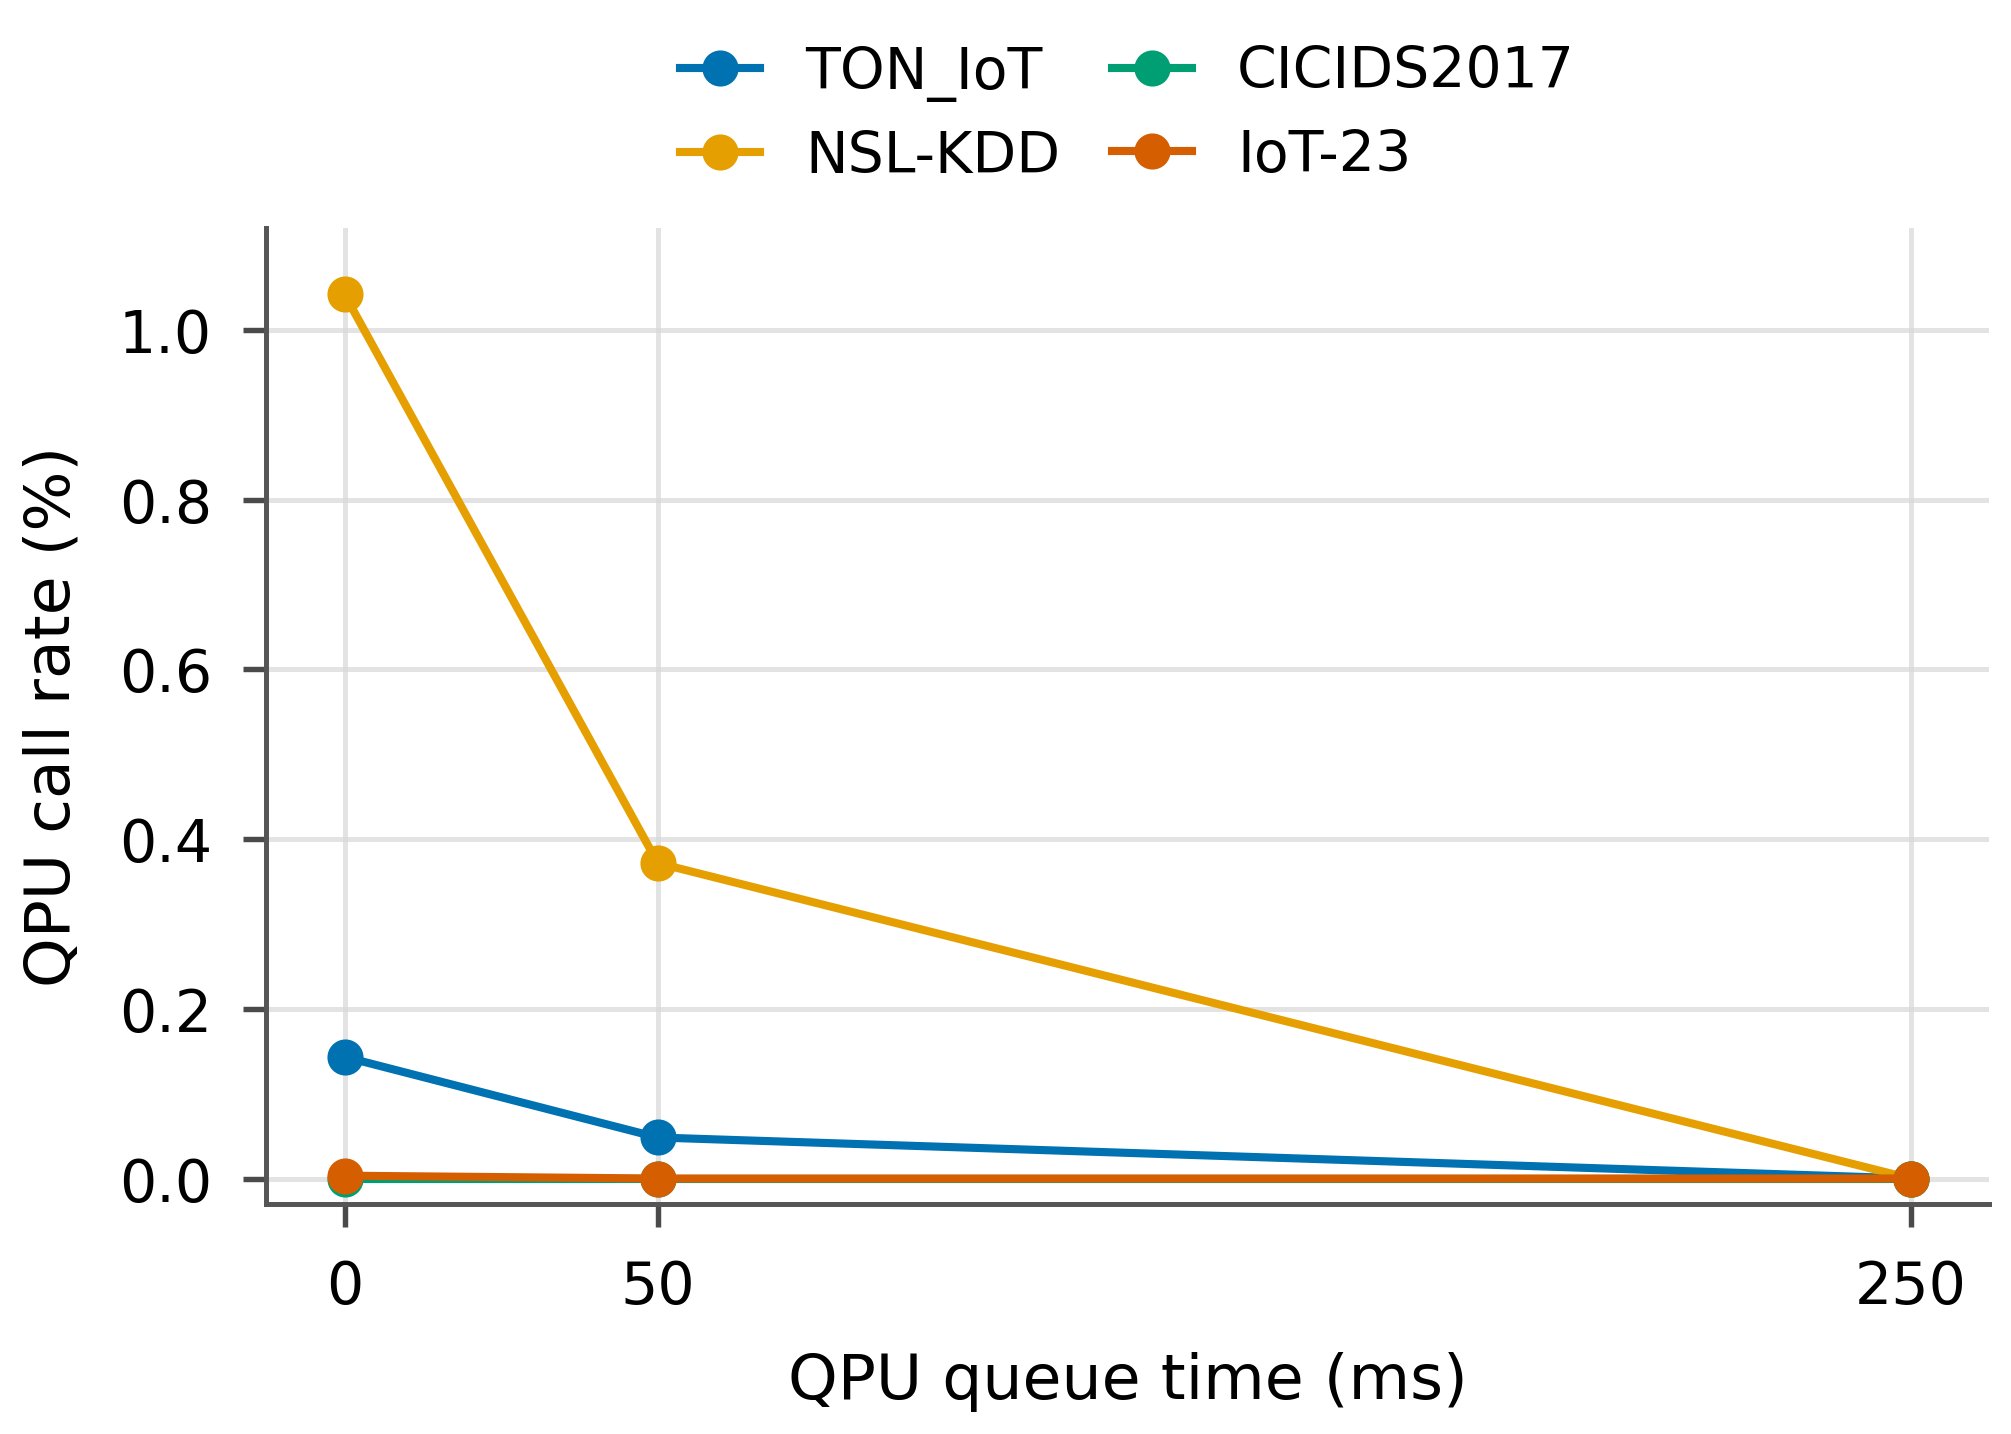
\includegraphics[width=\columnwidth]{figures/scheduler_qpu_call_rate_queue_sensitivity.png}
\caption{Queue-time sensitivity. HERO-S reduces QPU-capable routing as wait time increases.}
\label{fig:queue}
\end{figure}

This behavior clarifies how HERO-S differs from static QPU routing. Static QPU routing is insensitive to queue time, so its latency and EDP grow directly with the assumed wait. HERO-S uses queue time inside the score function and changes route decisions before the wait dominates the task. Even with lower modeled QPU energy, a 250 ms backend queue would exceed the 2.5 ms average gateway budget, so queue latency alone is sufficient to shift these tasks to classical routes.

\subsection{Qiskit Subset}
\begin{table}[t]
\caption{Qiskit quantum-kernel subset validation.}
\label{tab:qiskit}
\centering
\scriptsize
\resizebox{\columnwidth}{!}{%
\begin{tabular}{llcccc}
\toprule
Dataset & Variant & Train/test & Acc. & F1 & Runtime(s) \\
\midrule
TON\_IoT & noiseless & 16/8 & 0.833$\pm$0.072 & 0.804$\pm$0.120 & 10.38$\pm$0.52 \\
TON\_IoT & noisy\_low & 16/8 & 0.833$\pm$0.072 & 0.804$\pm$0.120 & 4.23$\pm$0.17 \\
NSL-KDD & noiseless & 16/8 & 0.833$\pm$0.072 & 0.821$\pm$0.062 & 10.90$\pm$0.31 \\
NSL-KDD & noisy\_low & 16/8 & 0.833$\pm$0.072 & 0.821$\pm$0.062 & 4.41$\pm$0.08 \\
\bottomrule
\end{tabular}}
\end{table}

The Qiskit subset serves as an implementation-feasibility check. Accuracy is quantized because each run uses only eight balanced test samples; the same 6/7/7-correct pattern across three seeds yields the identical 0.833$\pm$0.072 accuracy for both datasets even though F1 differs by class-error mix. The identical noiseless and low-noise labels on these tiny subsets indicate that the injected simulator noise did not flip the final SVM decision for the sampled points. The equality is treated as a small-sample artifact; accuracy and efficiency assessment of QPU routes requires larger hardware-backed quantum-kernel studies.

\section{Discussion}
HERO-S provides constrained route selection for an AIoT security pipeline. The empirical result concerns scheduling behavior: under an average gateway-latency budget, HERO-S improves over the closest uncertainty cascade, adapts to backend queue time, and allocates lower-utility QPU-capable tasks to classical routes. Cloud-only inference remains the upper-quality reference for deployments that can tolerate its latency and energy cost. At 250 ms queue time, the utility model assigns zero traffic to the QPU-capable path because the proxy quality and queue cost make classical routes preferable; at zero queue, Fig.~\ref{fig:queue} shows nonzero QPU-capable routing on TON\_IoT and NSL-KDD. The same utility and confidence gates can admit improved QPU kernels or shorter backend queues without changing the orchestration interface.

For deployment, the scheduler can run at an edge gateway or site controller because it requires only normalized flow features, model confidence, metadata, and backend telemetry. The policy is also auditable: each escalation can be explained by uncertainty, alert severity, asset criticality, confidence margin, queue time, and remaining latency budget. This is important for AIoT security operations where a controller alert, botnet flow, and low-risk sensor event should not consume accelerator resources in the same way. The fixed weights and gates used here are intentionally kept constant across datasets, so the reported gains are not produced by per-dataset retuning. In a production system, those weights could be calibrated against operator costs for false negatives, false positives, cloud usage, and remote accelerator access.

The energy model uses a fixed route-cost table. Edge and cloud energy are measured when RAPL/NVML counters are available and otherwise use the labeled fallback route model; in this paper the per-route values are fixed stress-test costs rather than dataset-specific power traces. QPU infrastructure energy is modeled because per-job facility telemetry is unavailable. These values stress-test route selection under remote-accelerator assumptions in which frequent QPU calls would be impractical for AIoT deployment.

The current implementation has limits. The QPU-compatible route is a reduced-kernel proxy at scheduler scale; the Qiskit subset is small; IoT-23 is comparatively easy after leakage-field removal; and real per-job QPU facility energy is unavailable. These limits motivate future work with larger hardware-backed quantum-kernel runs, online traffic replay, and deployment on an edge gateway connected to cloud inference and live quantum backends. The artifact is intended to support such extensions: the route interface only requires predicted quality, confidence, latency, energy, and queue state, so additional detectors or hardware backends can be added without changing the scheduler abstraction.

A representative operational path is as follows. A gateway first normalizes a flow record and runs the edge LR detector. If the edge model is confident and the asset is low criticality, HERO-S keeps the task local and avoids remote cost. If the same uncertainty occurs on a high-criticality controller or an alert with high false-negative cost, the scheduler evaluates cloud and QPU-capable routes. The cloud route is admitted only when the RF confidence and average-latency budget remain feasible. The QPU-capable route must also overcome queue, energy, and confidence penalties; otherwise it is explicitly bypassed. This path is intentionally simple to audit: every nonlocal decision can be traced to a small set of numeric fields rather than an opaque service-placement rule.

This structure also separates orchestration policy from classifier choice. The edge model could be replaced by a compact tree, linear SVM, or tiny neural detector; the cloud route could use a deeper ensemble or GPU model; and the QPU-capable route could be upgraded from the reduced-kernel proxy to a hardware-backed kernel. In each case, HERO-S needs the same route contract: estimated confidence, latency, energy, queue state, and expected quality gain. The reported experiments therefore evaluate the scheduling interface under current proxy quality, while leaving a clear path for stronger detectors and backends.


\section{Related Work}
\textit{IDS datasets and metrics.} AIoT intrusion detection requires datasets and metrics beyond accuracy because false negatives and false positives have different operational costs. Recent AIoT and industrial IoT security surveys emphasize heterogeneous devices, edge analytics, and AI-based defenses as deployment concerns \cite{siam2025aiot,alotaibi2023iiotsecurity}. TON\_IoT, IoT-23, CICIDS2017, and NSL-KDD cover complementary IoT, botnet, enterprise-flow, and legacy benchmark settings \cite{alsaedi2020toniot,garcia2020iot23,sharafaldin2018toward,tavallaee2009kdd}. HERO-S uses these datasets to evaluate routing policies rather than a single classifier, and reports FPR, FNR, PR-AUC, route-call rates, latency, and energy in addition to F1.

\textit{Deep-learning and IoT IDS.} Deep IDS surveys show that neural and ensemble models can perform well but must be benchmarked against strong classical baselines \cite{ferrag2020deep}. Online and IoT-specific systems such as Kitsune and N-BaIoT use autoencoder-style anomaly detection for network traffic and botnet detection \cite{mirsky2018kitsune,meidan2018nbaiot}. Software-defined, federated, and cloud-edge IoT IDS work studies multi-stage and distributed detection pipelines \cite{li2019sdiotids,nguyen2019diot,mothukuri2021survey,yang2023cloudedgeids}. HERO-S is orthogonal to these classifiers: it can route any detector family, but evaluates whether stronger routes justify extra delay and energy.

\textit{Edge-cloud orchestration.} Edge computing, MEC, and computation-offloading studies motivate placing latency-sensitive computation near devices and escalating selectively to cloud resources \cite{shi2016edge,mach2017mec,satyanarayanan2017edge,mao2017mec}. Edge-intelligence, energy-aware scheduling, and ML energy-accounting studies further motivate reporting quality together with cost metrics \cite{zhou2019edgeintelligence,chen2023energy,strubell2019energy}. Existing orchestrators typically optimize service placement, resource utilization, or communication delay. HERO-S focuses on a security-specific layer above those systems by combining IDS uncertainty, alert severity, asset criticality, false-negative risk, accelerator energy, and QPU queue time in one route utility.

\textit{Quantum-aware security workflows.} Hybrid quantum-classical learning studies motivate quantum feature maps, quantum kernels, and variational workflows \cite{havlicek2019supervised,schuld2019qml,cerezo2021vqa}; early security studies explore quantum machine learning for intrusion detection but remain limited in scale \cite{kalinin2023qmlids}. HERO-S treats these methods as optional candidate routes whose use must be justified by security utility, latency, queue time, confidence, and modeled energy. Queue-aware fallback for a low-quality QPU proxy is therefore part of the route-selection policy.

\section{Conclusion}
HERO-S is a QPU-aware energy-latency orchestration framework for AIoT intrusion detection. The evaluation shows that unconstrained cloud IDS remains the best quality reference, while HERO-S is effective under gateway budgets where cloud-only execution is infeasible. At 250 ms QPU queue time, HERO-S improves over edge-only and over a closest uncertainty-cascade baseline on TON\_IoT, NSL-KDD, and CICIDS2017, maintains the near-perfect IoT-23 edge result, reduces energy relative to cloud-only execution, and assigns QPU-capable tasks to classical routes when queue and utility conditions favor that choice. The central contribution is an auditable scheduling policy for deciding when QPU-capable execution is used, deferred, or avoided.

\bibliographystyle{IEEEtran}
\bibliography{references}
\end{document}
